% mnras_template.tex
%
% LaTeX template for creating an MNRAS paper
%
% v3.0 released 14 May 2015
% (version numbers match those of mnras.cls)
%
% Copyright (C) Royal Astronomical Society 2015
% Authors:
% Keith T. Smith (Royal Astronomical Society)

% Change log
%
% v3.0 May 2015
%    Renamed to match the new package name
%    Version number matches mnras.cls
%    A few minor tweaks to wording
% v1.0 September 2013
%    Beta testing only - never publicly released
%    First version: a simple (ish) template for creating an MNRAS paper

%%%%%%%%%%%%%%%%%%%%%%%%%%%%%%%%%%%%%%%%%%%%%%%%%%
% Basic setup. Most papers should leave these options alone.
\documentclass[fleqn,usenatbib]{mnras}

% MNRAS is set in Times font. If you don't have this installed (most LaTeX
% installations will be fine) or prefer the old Computer Modern fonts, comment
% out the following line
\usepackage{newtxtext,newtxmath}
% Depending on your LaTeX fonts installation, you might get better results with one of these:
%\usepackage{mathptmx}
%\usepackage{txfonts}

% Use vector fonts, so it zooms properly in on-screen viewing software
% Don't change these lines unless you know what you are doing
\usepackage[T1]{fontenc}
\usepackage{ae,aecompl}


%%%%% AUTHORS - PLACE YOUR OWN PACKAGES HERE %%%%%

% Only include extra packages if you really need them. Common packages are:
\usepackage{graphicx} % Including figure files
\usepackage{amsmath} % Advanced maths commands
\usepackage{xcolor} % Colour text for draft

%%%%%%%%%%%%%%%%%%%%%%%%%%%%%%%%%%%%%%%%%%%%%%%%%%

%%%%% AUTHORS - PLACE YOUR OWN COMMANDS HERE %%%%%

% Please keep new commands to a minimum, and use \newcommand not \def to avoid
% overwriting existing commands. Example:
%\newcommand{\pcm}{\,cm$^{-2}$} % per cm-squared
\newcommand{\dd}{\mathrm{d}}

% Use bold font for vectors
\let\vec\mathbf

%%%%%%%%%%%%%%%%%%%%%%%%%%%%%%%%%%%%%%%%%%%%%%%%%%

%%%%%%%%%%%%%%%%%%% TITLE PAGE %%%%%%%%%%%%%%%%%%%

% Title of the paper, and the short title which is used in the headers.
% Keep the title short and informative.
\title[SPH for multigrain dust]{A smoothed particle hydrodynamics algorithm for
multigrain dust with separate sets of particles}

% The list of authors, and the short list which is used in the headers.
% If you need two or more lines of authors, add an extra line using \newauthor
\author[Mentiplay, Price, \& Pinte]{%
   \parbox{\textwidth}{%
      Daniel Mentiplay\(^{1}\)\thanks{daniel.mentiplay@monash.edu},
      Daniel J. Price\(^{1}\),
      Christophe Pinte\(^{1,2}\)
   }\\
   \(^{1}\)Monash Centre for Astrophysics (MoCA) and School of Physics and
   Astronomy, Monash University, Clayton Vic 3800, Australia \\
   \(^{2}\)Univ. Grenoble Alpes, CNRS, IPAG, F-38000 Grenoble, France
}

% These dates will be filled out by the publisher
\date{Accepted XXX. Received YYY; in original form ZZZ}

% Enter the current year, for the copyright statements etc.
\pubyear{2020}

% Don't change these lines
\begin{document}
\label{firstpage}
\pagerange{\pageref{firstpage}--\pageref{lastpage}}
\maketitle

% Abstract of the paper
\begin{abstract}
   We present a new method for simulating the dynamics of a mixture of gas and
   multiple species of large Stokes number dust grains, typical of evolved
   protoplanetary discs and debris discs. The method improves upon earlier
   methods, in which only a single grain size could be represented, by capturing
   the differential backreaction of multiple dust species on the gas. This
   effect is greater for large dust-to-gas ratios that may be expected in the
   later stages of the protoplanetary disc life.
\end{abstract}

% Select between one and six entries from the list of approved keywords.
% Don't make up new ones.
\begin{keywords}
hydrodynamics -- methods: numerical -- protoplanetary discs
\end{keywords}

%%%%%%%%%%%%%%%%%%%%%%%%%%%%%%%%%%%%%%%%%%%%%%%%%%

%%%%%%%%%%%%%%%%% BODY OF PAPER %%%%%%%%%%%%%%%%%%

\section{Introduction}

Multi-wavelength observations of protoplanetary discs show that the radial
extent of the dust disc scales inversely with wavelength
\citep{Andrews2015PASP..127..961A}. This suggests that larger grains drift
inwards faster than smaller grains \citep{Weidenschilling1977MNRAS.180...57W}.

Modelling this requires dust and gas hydrodynamics with multiple dust
species---one of the grand challenges in protoplanetary disc modeling
\citep{Haworth2016PASA...33...53H}. In particular, it is important to capture
the collective backreaction of multiple dust species on the gas. For example,
the inward drift of small grains can be reversed by the inward drift of large
grains.

Grains of multiple sizes emit at the same wavelength. In order to interpret dust
continuum emission, for example in ALMA observations showing gaps and rings
\citep{ALMAPartnership2015ApJ...808L...3A, Andrews2016ApJ...820L..40A}, we must
model planet-disc interactions including multiple species. In particular,
interpretation of spectral index maps of discs with gaps requires models with
multiple dust species. Spectral index maps can put constraints on the size
distribution of dust grains within gaps \citep{Huang2018ApJ...852..122H}.
Multi-species dust models allow us to test the underlying disc models by
producing synthetic spectral index maps to compare with observations.

Discs containing dust asymmetries and spiral arms around central cavities can
show greater concentration at different wavelengths. Previous work has suggested
that the cause of these features is a (possibly unseen) companion in the cavity
\citep{Price2018MNRAS.477.1270P, Poblete2019MNRAS.489.2204P}. The ability to
perform multi-wavelength synthetic observations in single species dust-gas
hydrodynamical models is compromised. One option is to stack, in
post-processing, multiple single dust species simulations. However, due to back
reaction, there may be a phase difference in the location of the concentration
making this procedure unreliable.

There are two approaches to modelling of dust-gas mixtures in SPH: (i) the dust
and gas are represented by separate sets of SPH particles
\citep{Monaghan1995CoPhC..87..225M, Laibe2012MNRAS.420.2345L,
Laibe2012MNRAS.420.2365L}. In this approach the dust and gas SPH particles
interact via a drag coupling term. In the other approach, (ii) the dust and gas
are modelled by a single set of SPH particles representing the mixture
\citep{Price2015MNRAS.451..813P}. In this approach the dust fraction is stored
on the particles and evolved in time.

In the description for both of these approaches the methods are applicable to a
single species of dust with fixed size. \citet{Laibe2014MNRAS.444.1940L}
described a multiple species approach for the single SPH fluid method.
\citet{Hutchison2018MNRAS.476.2186H} provided an algorithmic implementation of
this method and tested this in the \textsc{Phantom} SPH code
\citep{Price2018PASA...35...31P}.

In this paper we extend method (i), in which dust is represented by separate
sets of particles, from a single species to multiple species. We present the
continuum equations to solve in Section~\ref{subsec:continuum}, and the SPH
discretisation of those equations in Section~\ref{subsec:sph}. We describe
several tests of the method, as implemented in \textsc{Phantom}, in
Section~\ref{sec:tests}. We discuss some of the challenges of the method in
Section~\ref{sec:discussion}.

\section{Methods}

\subsection{Continuum equations for multiple dust species}%
\label{subsec:continuum}

We consider a mixture of gas, indexed by \(g\), and \(N\) dust species, indexed
by \(d_i\). We neglect the finite size of the dust particles, and thus set the
gas volume fraction to unity. We represent each dust species as a continuous
fluid with a fixed size, \(s_i\), and intrinsic density, \(\varrho_{m_i}\).
Then, the equations of conservation of mass for the mixture is given by
%
\begin{align}
   \label{eqn:conserve-gas-mass}
   \frac{\partial \rho_g}{\partial t} + \nabla \cdot (\rho_g \vec{v}_g) &= 0, \\
   \label{eqn:conserve-dust-mass}
   \frac{\partial \rho_{d_i}}{\partial t} + \nabla \cdot (\rho_{d_i} \vec{v}_{d_i}) &= 0,
\end{align}
%
for each \(i\) in 1 to \(N\), where \(\rho_j\) and \(\vec{v}_j\) are the density
and velocity of the fluids.

We assume the fluids are inviscid, that the dust is pressureless, and that each
dust species is homogeneous, i.e.\ has the same mass, size, and intrinsic
density. The equations of conservation of momentum for the mixture are given by
%
\begin{align}
   \rho_g \frac{\dd \vec{v}_g}{\dd t}
      &= - \nabla P + \rho_g \vec{f} + \sum_i K_i \left(\vec{v}_{d_i}
         - \vec{v}_{g}\right), \\
   \rho_{d_i} \frac{\dd \vec{v}_{d_i}}{\dd t}
      &= \rho_{d_i} \vec{f} - K_i \left(\vec{v}_{d_i} - \vec{v}_{g}\right),
\end{align}
%
where \(P\) is the gas pressure, \(\vec{f}\) is any body forces acting on the
fluids, typically gravity from a star or planet (we ignore self-gravity in this
paper), and \(K_i\) is the drag coefficient between the gas and a particular
dust species, \(i\). Note that each dust fluid has one gas drag interaction
term, whereas the gas momentum equation has a sum of interactions over each dust
species. Also note that the dust has no pressure gradient force term. In
general, the drag coefficient could be a complicated expression. We assume that
the drag coefficient is linear with respect to the differential velocity,
\(\Delta \vec{v}_i = \vec{v}_{d_i} - \vec{v}_g \).

The gas and dust exchange momentum via drag which leads to frictional heating.
Under the assumption that the gas and dust grains are at the same temperature,
the evolution of gas internal energy is given by
%
\begin{align}
   \label{eqn:conserve-energy}
   \rho_g \frac{\dd u_g}{\dd t} =
      - P \nabla \cdot \vec{v}_g + \rho_g \sum_i K_i {(\vec{v}_g - \vec{v}_{d_i})}^2.
\end{align}
%
We neglect the dust fluid internal energy under the assumption that the dust and
gas are at the same temperature.

Equations~\ref{eqn:conserve-gas-mass}--\ref{eqn:conserve-energy} are \(2N + 3\)
equations describing the evolution of a mixture of gas and \(N\) dust species.
We discuss discretising these equations with smoothed particle hydrodynamics in
Section~\ref{subsec:sph}.

\subsection{Drag timescale}

\subsubsection{Drag coefficient and stopping time}

Dust and gas interact via a drag force. This drag force has a characteristic
time scale, known as the stopping time. The stopping time relates to the drag
coefficient, which depends on quantities such as the gas temperature and
density, and on the physical characteristics of the dust grains. For a single
dust species, the stopping time, \(t_s\), is given by
%
\begin{align}
   \label{eqn:single-stopping-time}
   t_s = \frac{\rho_g \rho_d}{K (\rho_g + \rho_d)},
\end{align}
%
where \(K\) is the drag coefficient for the single species. We assume spherical
grains of size \(s\) with a uniform material density, \(\varrho_m\). In the
linear Epstein regime \citep{Epstein1924PhRv...23..710E} the drag coefficient
\(K\) is
%
\begin{align}
   \label{eqn:single-drag-coefficient}
   K = \frac{\rho_g \rho_d}{\varrho_m s} \sqrt{\frac{8}{\pi\gamma}} c_s f,
\end{align}
%
where \(\gamma\) is the adiabatic index of the gas. For convenience, we define
an effective material density, \(\varrho_{\mathrm{eff}}\), given by
\(\varrho_{\mathrm{eff}} = \varrho_m \sqrt{\pi\gamma/8}\). In addition, \(f\) is
a correction for supersonic relative velocities given by
\citep{Kwok1975ApJ...198..583K}
%
\begin{align}
   \label{eqn:supersonic}
   f = \sqrt{1 + \frac{9\pi}{128}} \frac{\Delta v^2}{c_s^2}.
\end{align}
%

As discussed in \citet{Hutchison2018MNRAS.476.2186H}, a straightforward
generalisation of the stopping time for multiple dust species is not available.
Each dust species is separately coupled to the gas by the drag force. However,
the dust species are indirectly coupled to each other via backreaction, as
required conservation of momentum. Considering the multiple dust species case,
and ignoring the supersonic correction factor, the drag coefficient, \(K_i\), is
now
%
\begin{align}
   \label{eqn:drag-coefficient}
   K_i = \frac{\rho_g \rho_{d_i} c_s}{\varrho_{\mathrm{eff}} s_i}.
\end{align}
%
In analogy with Equation~\ref{eqn:single-stopping-time} we can define a
``stopping time'', \(t'_{s_i}\), as
%
\begin{align}
   \label{eqn:alternative-stopping-time}
   t'_{s_i} = \frac{\rho_g \rho_{d_i}}{K_i (\rho_g + \rho_{d_i})}.
\end{align}
%
However, there are other ``stopping times'' we can define. First, we define
\(\rho = \rho_g + \sum_i \rho_{d_i}\) as the total density of the gas and all
dust species. Then we can define another ``stopping time'', \(t_{s_i}\), as
%
\begin{align}
   \label{eqn:stopping-time}
   t_{s_i} = \frac{\rho_g \rho_{d_i}}{K_i \rho}.
\end{align}
%
Considering the mixture of dust and gas as a whole, we define the weighted sum
\(s_{\mathrm{eff}} = \sum_i \rho_{d_i} s_i / \sum_i \rho_{d_i}\) as an effective
grain size for the mixture. Then we can define an effective stopping time for
the dust mixture as
%
\begin{align}
   \label{eqn:effective-stopping-time}
   T_s = \frac{\varrho_{\mathrm{eff}} s_{\mathrm{eff}}}{\rho c_s}.
\end{align}
%
By combining
Equations~\ref{eqn:single-stopping-time}~\&~\ref{eqn:single-drag-coefficient} we
can see the expression for the multigrain effective stopping time is analogous
to the single dust species case.

\subsubsection{Stokes number}

The Stokes number, \(\mathrm{St}\), is a dimensionless stopping time defined as
the stopping time in units of a typical flow time. For protoplanetary discs, the
typical flow time is the Keplerian orbital time, \(1/\Omega_K\), so that the
Stokes number is \(\mathrm{St} = t_s \Omega_K\). Note that the Stokes number
depends on the gas disc properties, via the density and temperature, the dust
disc density, the dust grain properties, i.e. size and material density, and the
stellar mass and orbital distance. The disc surface density, \(\Sigma\), and
disc scale height, \(H\), are related to the density, sound speed, and Keplerian
orbital time by \(\rho = \Sigma / H\) and \(\Omega_K = c_s / H\). Using these
relations we can show that the Stokes number in the midplane of a protoplanetary
disc is given by
%
\begin{align}
   \mathrm{St} = \frac{\varrho_{\mathrm{eff}} s}{\Sigma}.
\end{align}
%
In using \(\rho = \Sigma / H\) and \(\Omega_K = c_s / H\) to derived the above
expression we are assuming that the gas mass dominates over the dust mass, i.e.
that the dust fraction is low. Otherwise we must consider that the scale height
varies between the gas disc and the dust sub-discs.

Considering the multiple dust species case, we can define an effective midplane
Stokes number for the mixture using the effective stopping time
(Equation~\ref{eqn:effective-stopping-time}) as \(\mathrm{St}_{\mathrm{eff}} =
\varrho_{\mathrm{eff}} s_{\mathrm{eff}} / \Sigma \). An alternative is to define
a per species midplane Stokes number in analogy with the single grain size case:
%
\begin{align}
   \label{eqn:stokes}
   \mathrm{St}_i = \frac{\varrho_{\mathrm{eff}} s_i}
      {\Sigma_g \left(1 + \sum_i \varepsilon_i \right)},
\end{align}
%
where \(\Sigma_g\) is the gas surface density and \(\varepsilon_i\) is the
dust-to-gas ratio for each dust species. Again we see the combination of grain
properties, size and material density, and the disc surface density fixing the
Stokes number. Given that we assume the material density is the same for all
species, we see that the grain size of the species, for any fixed location in
the disc, gives the variation in Stokes number between species.

The Stokes number controls the dynamics of dust grains in protoplanetary discs
\citep{Weidenschilling1977MNRAS.180...57W,Takeuchi2002ApJ...581.1344T},
affecting radial drift, vertical settling, and gap and spiral formation. The
individual Stokes number (Equation~\ref{eqn:stokes}) encapsulates the dynamics
of each dust species. We can distinguish between three regimes of dust dynamics:
%
\begin{enumerate}
   \item small grains, i.e.\ those with \(\mathrm{St} \ll 1\),
   \item large grains, i.e.\ those with \(\mathrm{St} \gg 1\), and
   \item intermediate-sized grains, i.e.\ those with \(\mathrm{St} \sim 1\).
\end{enumerate}
%
Small grains have short stopping time, i.e.\ differential velocity decays on
less than the orbital time, and are thus strongly coupled to the gas. These
grains stick to the gas, e.g.\ following the gas accretion flow. Large grains
have long stopping time, i.e.\ differential velocity decays on timescales much
longer than the orbital time, and are thus weakly coupled to the gas.
Intermediate-sized grains are marginally coupled to the gas. These grains
experience the fastest radial drift velocities
\citep{Takeuchi2002ApJ...581.1344T,Ayliffe2012MNRAS.423.1450A}. For a typical
protoplanetary disc, with surface density \(\approx 1\)~g cm\({}^{-2}\),
small grains are \(\lesssim 10 \mu\mathrm{m}\), and large grains are \(\gtrsim 1
\mathrm{mm}\). Note that for other physical systems the terms small and large
grains have different meaning. For example, in the ISM large grains might be any
grains \(> 10 \mu\mathrm{m}\).

Several works describe the behaviour of these dust species as independently
coupled to the gas
\citep{Nakagawa1986Icar...67..375N,Dipierro2017MNRAS.469.1932D,Kanagawa2017ApJ...844..142K}.
\citet{Dipierro2018MNRAS.479.4187D} extend the analysis to consider the full
backreaction of all species onto the gas. They show that the cumulative
backreaction from multiple dust species can strongly affect the gas flow, even
for low dust-to-gas ratio, and that, for large dust-to-gas ratio, the large
grains can drift outwards, as opposed to the typical inwards drift. This gives
motivation to the current work.


\subsection{SPH with multiple dust species}%
\label{subsec:sph}

\subsubsection{SPH density with multiple dust species}

We extend the SPH method for dust and gas mixtures with a single species, first
described in \citet{Monaghan1995CoPhC..87..225M} and improved upon by
\citet{Laibe2012MNRAS.420.2345L,Laibe2012MNRAS.420.2365L}, to multiple dust
species. We use a separate set of particles to represent the gas and each dust
species. So each phase of the mixture has its own density and smoothing length
which depend only on the neighbouring particles of its own phase. This differs
from the 1-fluid method described by \citet{Hutchison2018MNRAS.476.2186H} in
which there is a single set of SPH particles representing the mixture. The SPH
formulation of the continuity equations,
Equations~\ref{eqn:conserve-gas-mass}--\ref{eqn:conserve-dust-mass}, are given
by
%
\begin{align}
   \label{eqn:sph-density}
   \rho^k_a &= \sum_b m^k_b W_{ab}(h^k_b), \\
   h^k_a &= \eta \left(\frac{m^k_a}{\rho^k_a}\right)^{1/\nu},
   \label{eqn:sph-smoothing}
\end{align}
%
where the superscript \(k \in \{g, d_1, \dots, d_N\}\) is an index
distinguishing between the gas and all dust species; \(\nu\) is the number of
spatial dimensions; \(m^k_a\), \(\rho^k_a\) and \(h^k_a\) are the SPH particle
mass, density, and smoothing length, respectively; \(W_{ab}\) is the SPH
smoothing kernel; and \(\eta\) is a factor of order unity which determines the
number of neighbours per particle. For an overview on the SPH method, see:
\citet{Monaghan1992ARA&A..30..543M,Price2012JCoPh.231..759P}  So there are \(N +
1\) sets of equations, Equations \ref{eqn:sph-density}--\ref{eqn:sph-smoothing},
one set per phase. This is a straightforward generalisation of previous single
dust species methods.

One important feature of the above equations is that the gas and dust densities
(for each dust species) are calculated without reference to any other phase.
Given that the dust is pressureless this can lead to dust becoming trapped under
the gas resolution. This is in contrast to the gas in which, due to the pressure
force, particles are kept apart to prevent this over-concentration. Dust and gas
interact only via drag which requires relative motion. If dust particles become
concentrated and remain motionless with respect to the local gas distribution
there is no pressure force to stop further collapse. This can lead to unphysical
clumping of dust which can mimic physical clumping of dust that might be
expected, in, for example, protoplanetary discs.

\subsubsection{SPH equation of motion with multiple dust species}

The equations of motion in SPH can be derived from a Lagrangian giving exact
conservation of linear and angular momentum, and energy
\citep{Price2012JCoPh.231..759P}. Following \citet{Laibe2012MNRAS.420.2345L},
the equation of motion for the gas is given by
%
\begin{align}
   \label{eqn:sph-gas-velocity}
   \begin{split}
      \frac{\dd \vec{v}^g_a}{\dd t} = &- \sum_{b \in g} m^g_b \left[
         \frac{P_a}{\Omega^g_a {\left(\rho^g_a\right)}^2} \nabla_a W_{ab}(h^g_a) +
         \frac{P_b}{\Omega^g_b {\left(\rho^g_b\right)}^2} \nabla_a W_{ab}(h^g_b)
      \right] \\
      &+ \nu \sum_{i=1}^N \sum_{b \in d_i} m^g_b \frac{K_{ab}}{\rho^g_a \rho^{d_i}_b}
         (\vec{v}_{ab} \cdot \hat{\vec{r}}_{ab}) \hat{\vec{r}}_{ab} D_{ab}(h^g_a),
   \end{split}
\end{align}
%
where \(P_a\) refers to the pressure on particle \(a\), and \(\Omega^g_a\) is a
term related to the variable smoothing length given by
%
\begin{align}
   \Omega^g_a = 1 - \frac{\partial h_a}{\partial \rho_a}
      \sum_b m_b \frac{\partial W_{ab}(h_a)}{\partial h_a}.
\end{align}
%
The equation of motion for each dust species, \(d_i\), is given by
%
\begin{align}
   \label{eqn:sph-dust-velocity}
   \frac{\dd \vec{v}^{d_i}_a}{\dd t} =
      - \nu \sum_{b \in g} m^{d_i}_b \frac{K_{ab}}{\rho^g_b \rho^{d_i}_a}
      (\vec{v}_{ab} \cdot \hat{\vec{r}}_{ab}) \hat{\vec{r}}_{ab} D_{ab}(h^g_b),
\end{align}
%
The first term in Equation~\ref{eqn:sph-gas-velocity} represents the usual SPH
discretisation of the pressure gradient force on a particle, labelled by \(a\).
The sum, denoted by \(\sum_{b \in g}\), is a sum over gas neighbours, labelled
by \(b\).

\subsubsection{Drag kernel and drag coefficient}

The second term in Equation~\ref{eqn:sph-gas-velocity} represents the cumulative
drag force from each dust species on particle \(a\) (with \(i \in \{1, \ldots,
N\}\) representing each species). For each species, the sum, denoted by
\(\sum_{b \in d_i}\), is a sum over dust neighbours, labelled by \(b\). The
terms \(K_{ab}\), \(\vec{v}_{ab}\), and \(\hat{\vec{r}}_{ab}\) are the drag
coefficient, relative velocity, and a unit vector in the direction of the
displacement vector, between the particles, where here the \(a\) index refers to
the gas particle and the \(b\) index refers to its dust neighbours. Similarly,
the sum on the right hand side of Equation~\ref{eqn:sph-dust-velocity}
represents the drag force from the gas on the particular dust species, where
\(a\) refers to a dust (SPH) particle and \(b\) refers to its gas neighbours.

Equations~\ref{eqn:sph-gas-velocity} and~\ref{eqn:sph-dust-velocity} are a
straightforward generalisation of \citet{Laibe2012MNRAS.420.2345L} to multiple
dust species. For Epstein drag, the drag coefficient \(K_{ab}\) is given by
%
\begin{align}
   K_{ab} = \frac{\rho^g_a \rho^{d_i}_b}{\varrho_{\mathrm{eff}} s_i} c_{s,a} f_{ab},
\end{align}
%
where \(c_{s,a}\) is the sound speed on the gas particle and \(f_{ab}\)
supersonic correction factor (Equation~\ref{eqn:supersonic}) between the two
particles.

The typical bell-shaped kernel used in SPH to estimate density (denoted by
\(W_{ab}\)) is not appropriate for the drag force summation. Rather, a
`double-hump' kernel is appropriate \citep{Laibe2012MNRAS.420.2345L}. I.e.\ a
kernel that is an even function with two maxima and a zero in the middle.

\subsection{Time stepping}

\subsubsection{Time step constraint}

We use an explicit leapfrog time stepping scheme as discussed in
\citet{Price2018PASA...35...31P}. Given that we use an explicit scheme for the
drag term there is an additional stability constraint on the timestep \(\Delta
t\). We derive this constraint for the forward Euler scheme. (Even though we do
not use this scheme, it provides a guide to the nature of the constraint.)
Starting with the discretisation of the drag-only velocity equations for dust
and gas with the forward Euler method, we have
%
\begin{align}
   \frac{v_g^{n+1} - v_g^n}{\Delta t} &= - \sum_i \frac{K_i}{\rho_g} \left(v_g^n - v_{d_i}^n\right), \\
   \frac{v_{d_i}^{n+1} - v_{d_i}^n}{\Delta t} &= \frac{K_i}{\rho_{d_i}} \left(v_g^n - v_{d_i}^n\right).
\end{align}
%
Then we perform a von Neumann stability analysis, where we expand the solution
in plane waves, \(v_j^m = V_j^m e^{i k x}\), where \(j\) refers to the species,
\(k\) is the wavenumber, and \(m\) refers to the time step. This expansion leads
to the following matrix equation:
%
\begin{align}
   \begin{pmatrix}
      V_g \\ V_{d_1} \\ \vdots \\ V_{d_N} \\
   \end{pmatrix}^{n+1} =
   \begin{pmatrix}
      1 - \frac{\Delta t \sum K_i}{\rho_g} & \frac{\Delta t K_1}{\rho_g} & \dots & \frac{\Delta t K_N}{\rho_g} \\
      \frac{\Delta t K_1}{\rho_{d_1}} & 1 - \frac{\Delta t K_1}{\rho_{d_1}} & \dots & 0 \\
      \vdots & \vdots & \vdots & \vdots \\
      \frac{\Delta t K_N}{\rho_{d_N}} & 0 & \dots & 1 - \frac{\Delta t K_N}{\rho_{d_N}} \\
   \end{pmatrix}
   \begin{pmatrix}
      V_g \\ V_{d_1} \\ \vdots \\ V_{d_N} \\
   \end{pmatrix}^{n}.
\end{align}
%
We find the characteristic polynomial of the matrix, \(M\), above using the
expression \(\det(M - \lambda I) = \det(A - B D^{-1} C) \det(D)\) to give
%
\begin{align}
   \left(1 - \frac{\Delta t \sum K_i}{\rho_g} - f - \lambda\right)
   \times \prod_i \left(1 - \frac{\Delta t K_i}{\rho_{d_i}} - \lambda\right),
\end{align}
%
where \(f = \sum_i \Delta t^2 K_i^2 \left[\rho_g \rho_{d_i} \left( 1 -
\frac{\Delta t K_i}{\rho_{d_i}} - \lambda \right) \right]^{-1}\). We neglect
\(f\) as it is second order in \(\Delta t\). To find the eigenvalues we equate
the characteristic polynomial with zero and solve to find
%
\begin{align}
   \lambda_g = 1 - \frac{\Delta t \sum_i K_i}{\rho_g} \quad \mathrm{and} \quad
   \lambda_{d_i} = 1 - \frac{\Delta t K_i}{\rho_{d_i}}.
\end{align}
%
For stability, we require \(|\lambda_k| < 1\). Using this condition with
Equations~\ref{eqn:drag-coefficient}~\&~\ref{eqn:stopping-time} gives the
following timestep criteria:
%
\begin{align}
   \Delta t < \frac{2}{\sum_i \epsilon_i / t_{s_i}} \quad {\rm and} \quad
   \Delta t < \frac{2 t_{s_i}}{1 - \epsilon} \quad \forall \, i,
\end{align}
%
where \(\epsilon = \sum_i \epsilon_i\) and \(\epsilon_i = \rho_{d_i} / \rho\).
We have \(N + 1\) inequalities. We take the minimum over dust stopping times in
the inequality on the right to find the most restrictive timestep criterion
involving only dust quantities:
%
\begin{align}
   \label{eqn:timestep-dust}
   \Delta t < \frac{2}{1 - \epsilon} \min_i t_{s_i}.
\end{align}
%
We can find an upper bound on the inequality involving the gas density by taking
the minimum over the dust fractions and maximum over the stopping times to give
%
\begin{align}
   \label{eqn:timestep-gas}
   \Delta t < \frac{2}{N} \frac{\max_i t_{s_i}}{\min_i \epsilon_i}.
\end{align}
%
This is a sufficient but not necessary condition. Given that \(N\) is of order
tens and, at worst, \(\min_i \epsilon_i \sim 1\), we can say that
Equation~\ref{eqn:timestep-dust} is more restrictive than
Equation~\ref{eqn:timestep-gas}, and thus provides the time step constraint for
drag. Note that (i) the stability constraint depends on the shortest stopping
time, and (ii) for large dust-to-gas ratios, i.e. \(\epsilon \rightarrow 1\),
the stability constraint becomes unimportant.

This timestep constraint is not the same as the one derived in
\citet{Laibe2012MNRAS.420.2345L} for a single dust species. In that case, the
time step constraint is the stopping time itself, and does not depend on the
dust fraction. Note that we have shown that Equation~\ref{eqn:timestep-dust} is
the stability constraint for the forward Euler discretisation of the drag terms
to first order in \(\Delta t\). However, we have not derived the stability
constraint for the leapfrog scheme we use in our numerical tests below.

\subsubsection{Time step constraint for SPH}

We can rewrite the time step constraint in Equation~\ref{eqn:stopping-time}
using the alternative stopping time
(defined in Equation~\ref{eqn:alternative-stopping-time}) as
%
\begin{align}
   \Delta t < 2 \min_i \{t'_{s_i} (1 + \varepsilon_i)\},
\end{align}
%
where \(\varepsilon_i = \rho_{d_i} / \rho_g\) is the dust-to-gas ratio for each
dust species. This is useful because in evolving the momentum equations we use
the drag coefficient on a dust (or gas) particle over its gas (or dust)
neighbours, without reference to the other dust species. Given that
\(\varepsilon_i > 0\), for simplicity, we take the more restrictive constraint of
setting \(\varepsilon_i = 0\), i.e.
%
\begin{align}
   \label{eqn:sph-timestep-constraint}
   \Delta t < 2 \min_i t'_{s_i}.
\end{align}
%
For a dust particle, we take the minimum over gas neighbours of the individual
species constraint (\(\Delta t < 2 t_{s_i}\)):
%
\begin{align}
   \Delta t < 2 \min_{a}
   \left\{ \frac{\rho^g_a \rho^{d_i}_b}{K_{ab} (\rho^g_a + \rho^{d_i}_b)} \right\}.
\end{align}
%
Whereas, for a gas particle, we take the minimum of
Equation~\ref{eqn:sph-timestep-constraint}, rewritten in terms of the drag
coefficient and densities, over the neighbouring dust particles to find the SPH
time step constraint for a particle:
%
\begin{align}
   \Delta t < 2 \min_i \min_{b}
   \left\{ \frac{\rho^g_a \rho^{d_i}_b}{K_{ab} (\rho^g_a + \rho^{d_i}_b)} \right\}.
\end{align}
%

\section{Numerical tests}%
\label{sec:tests}

We implemented the numerical method described in Section~\ref{subsec:sph} in the
smoothed particle hydrodynamics code \textsc{Phantom}\footnote{See the git
commit labelled by the hash \texttt{64dbd2b1} in the \textsc{Phantom} source
code repository for the implemented changes.}. We then performed several tests
to validate the method against known analytical solutions. The dusty box test
(Section~\ref{subsec:box}) validates the drag force coupling in the absence of
spatial gradients. The dusty wave test (Section~\ref{subsec:wave}) validates the
method with spatial gradients in a linear regime. The dusty shock test
(Section~\ref{subsec:shock}) validates the method in a challenging non-linear
regime.

The tests all have analytical solutions in one spatial dimension. We peformed
each of the tests in three dimensions, and then reduced the data to one
dimension for comparison with the analytical solutions. In each of the tests we
used, unless stated otherwise: a globally isothermal equation of state
(\texttt{ieos} = 1 in \textsc{Phantom}); the quintic kernel with 113 mean
particle neighbours (\texttt{hfact} = 1.0 in \textsc{Phantom}); global
timestepping, i.e., all particles have the same time step; a Courant factor of
0.3 (\texttt{C\_cour} in \textsc{Phantom}); a time step constraint on the
acceleration \( C_{\rm force} \) of 0.25, where \(\Delta t_a < C_{\rm force}
\sqrt{h_a / |\vec{a}_a|} \) (\texttt{C\_force} in \textsc{Phantom}).


\subsection{Dusty box}%
\label{subsec:box}

\begin{figure*}
   \begin{center}
      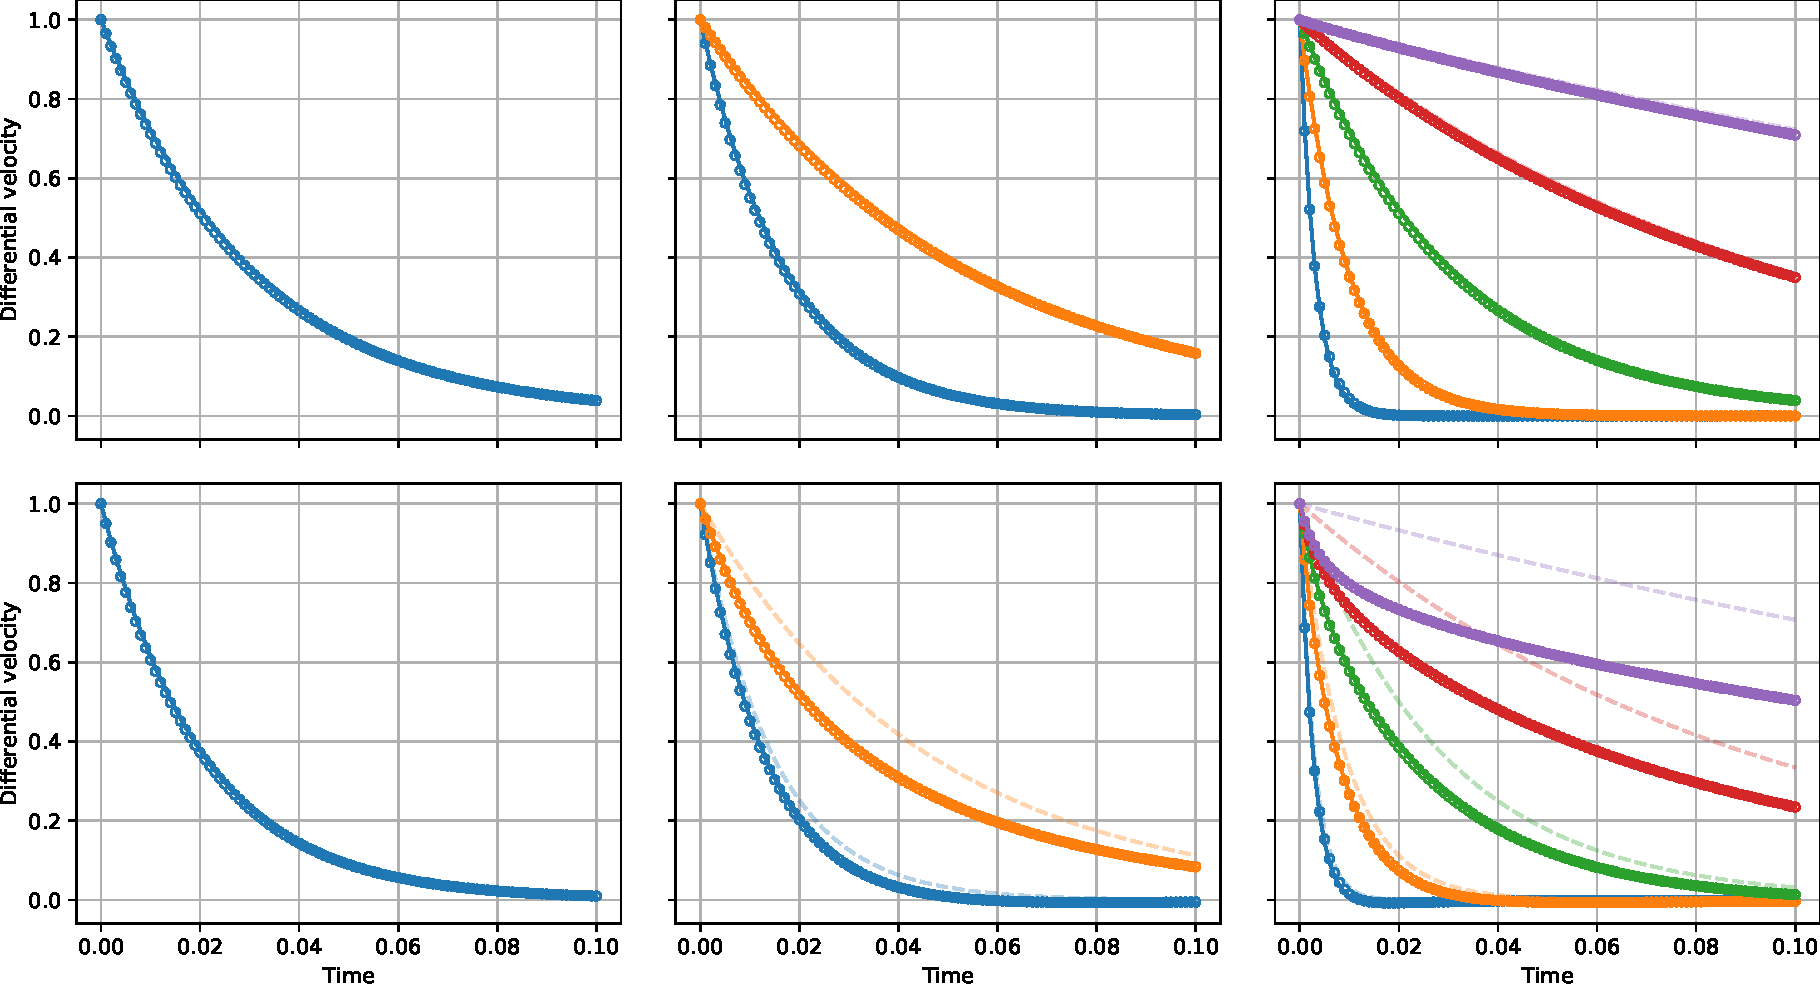
\includegraphics[width=\textwidth]{figs/dustybox_differential_velocity_comparison.pdf}
      \caption{Dusty box numerical test showing the differential velocity
         between the dust and gas. The total dust-to-gas ratio is 0.01 (top row)
         and 0.5 (bottom row). From left to right: the number of dust species is
         1, 2, 5. The open circles represent the results from the
         \textsc{Phantom} numerical solution. The solid and dashed lines
         represent the analytical solution with and without taking back reaction
         into account, respectively. In the top row, the solid and dash lines
         lie on top of each other. In the bottom row, the numerical solution
         matches the analytical solution including backreaction. Each colour
         represents the differential velocity of a dust species.%
         \label{fig:dustybox}}
   \end{center}
\end{figure*}

We performed the multigrain version of the dusty box test described in
\citet{Laibe2011MNRAS.418.1491L}. We set up a periodic box of uniform density
gas and dust with an initial differential velocity between the gas and each dust
species. In this test, the equation of motion simplifies to
%
\begin{align}
   \frac{\partial \Delta \vec{V}}{\partial t} = - \Omega \Delta \vec{V},
\end{align}
%
where \(\Delta \vec{V}\) is the differential velocity vector in the direction of
motion, i.e. \(\vec{v}_{d_i} - \vec{v}_g\) for each \(i\) projected along the
direction of motion, and \(\Omega\) is the drag matrix (Equation~65 of
\citet{Laibe2014MNRAS.444.1940L}) given by,
%
\begin{align}
   \Omega_{ij} =
   \begin{cases}
      \frac{1}{t''_{s_i}} \frac{1}{(1 - \varepsilon)}, &i \neq j,\\
      \frac{1}{t''_{s_i}} \left( \frac{1}{\varepsilon_i} +
         \frac{1}{1 - \varepsilon} \right), &i = j,
   \end{cases}
\end{align}
%
where \( \varepsilon = \sum_i \varepsilon_i \), and \( t''_{s_i} = \left( \sum_i
\rho_i \right) / K_i \).

\begin{table}
   \centering
   \begin{tabular}{ccc}
      \hline
      \hline
      Species & Grain size [cm] \\
      \hline
      \hline
      One dust species \\
      1 & 1.0 \\
      \hline
      Two dust species \\
      1 & 0.562 \\
      2 & 1.78 \\
      \hline
      Five dust species \\
      1 & 0.1 \\
      2 & 0.316 \\
      3 & 1.0 \\
      4 & 3.16 \\
      5 & 10.0 \\
      \hline
      \hline
   \end{tabular}
   \caption{Grain sizes for dusty box test.}%
   \label{tab:box}
\end{table}

This problem tests how well the numerical scheme captures the exchange of
momentum between gas and each dust species via the drag force. All tests were in
the linear Epstein drag regime. We performed six tests in two sets of three. The
first set had a total dust-to-gas ratio of 0.01, and the second set 0.5. The
tests within each set had 1, 2, and 5 dust species, respectively, with grain
sizes given in Table~\ref{tab:box}. Each test had equal mass in each grain size
bin. The gas is initially motionless, and each dust species has uniform velocity
in the positive x-direction. We turned off the SPH viscosity, i.e. set
\texttt{alpha} to zero in \textsc{Phantom}.

For each test problem, we set up each of the gas and dust fluids on a
close-packed lattice, such that there were 44928 gas particles (32 particles in
the direction of motion), and 5472 dust particles per species (16 particles in
the direction of motion). We set the gas density to
\(10^{-13}\)~g~cm\({}^{-3}\), with dust density varying per test problem. We set
the dust grain density to \(0.5 \times 10^{-14}\)~g~cm\({}^{-3}\).

Figure~\ref{fig:dustybox} shows the time evolution of the mean velocity
differential between the gas and each dust species, compared with analytical
solutions. Given that there are no spatial gradients in the problem, all
particles follow the mean velocity. The dashed lines represent the analytical
solution without backreaction from the dust on the gas. The solid lines
represent the analytical solution including backreaction.

For low dust-to-gas ratio (0.01) both analytical solutions give the same decay
of differential velocity, with which the \textsc{Phantom} simulation agrees. For
a larger dust-to-gas ratio (0.5) the analytical solutions diverge, and the
\textsc{Phantom} simulation data follows the backreaction-inclusive solution. In
all cases, the numerical solution matches the analytical solution with relative
error less than 0.01.

For large dust-to-gas ratio we see that the smaller grains (0.1 cm and 0.316 cm)
rapidly slow and the differential velocity reverses sign. I.e. the small grains
slow to the gas velocity; then, as the larger grains speed up the gas via drag,
the gas drags the small grains along with it. This shows that the behaviour of
multiple dust species for large dust-to-gas ratios requires taking back reaction
into consideration to capture the physics of dust drag accurately
\citep{Gonzalez2017MNRAS.467.1984G,Dipierro2018MNRAS.479.4187D}.

\subsection{Dusty wave}%
\label{subsec:wave}

\begin{figure*}
   \begin{center}
      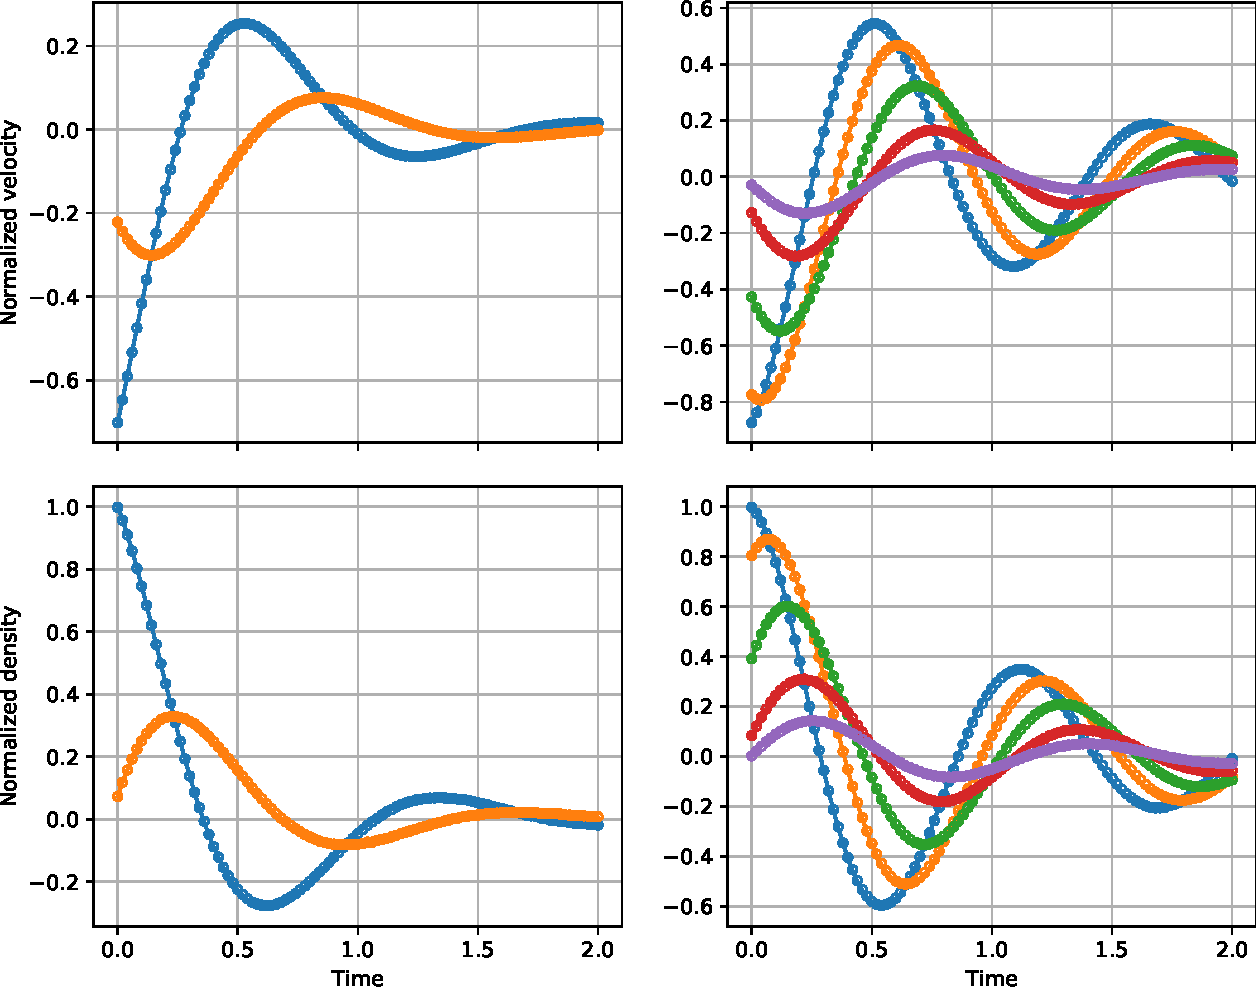
\includegraphics[width=0.66\textwidth]{figs/dustywave_velocity_density.pdf}
      \caption{Dusty wave numerical test showing the normalised velocity (top)
         and density (bottom) perturbation at \(x = 0\), for gas with one dust
         species (left) and gas with four dust species (right). The open circles
         represent the \textsc{Phantom} simulation, and the solid line
         represents the analytical solution from
         \citet{Benitez-Llambay2019ApJS..241...25B}. The gas is blue, and other
         colours represent different dust species.%
         \label{fig:dustywave}}
   \end{center}
\end{figure*}

We performed the multigrain version of the dusty wave test described in
\citet{Laibe2011MNRAS.418.1491L}. This is a test of the dust-gas drag coupling
in the context of a damped sound wave. The dust is a pressureless fluid and
cannot support sound waves. However, the gas can support sounds waves and drags
the dust. This leads to damping of the wave. This tests the numerical
method in a problem including spatial gradients in a linear regime.

Considering small perturbations around an equilibrium state, \(\rho_j = \rho_j^0
+ \delta \rho_j\), and \(v_j = \delta v_j\), where the index \(j\) is \(g\) for
the gas species, and \(d_i\) for each of the dust species, the linearised
equations of motion for this system are
%
\begin{align}
   \frac{\partial \delta \rho_g}{\partial t}
      + \rho_g^0 \frac{\partial \delta v_g}{\partial x} &= 0, \\
   \frac{\partial \delta \rho_{d_i}}{\partial t}
      + \rho_{d_i}^0 \frac{\partial \delta v_{d_i}}{\partial x} &= 0, \\
   \rho_g^0 \frac{\partial \delta v_g}{\partial t}
      &= \sum_i K_i \left(\delta v_{d_i} - \delta v_g \right)
         + c_s^2 \frac{\partial \delta \rho_g}{\partial x}, \\
   \rho_{d_i}^0 \frac{\partial \delta v_{d_i}}{\partial t}
      &= - K_i \left(\delta v_{d_i} - \delta v_{g}\right).
\end{align}
%
For the particular setup we followed \citet{Benitez-Llambay2019ApJS..241...25B}.
They derive solutions for the above equations as a dispersion relation (their
Equation~45) and associated set of eigenfunctions (their Equations~46--48).
Following \citet{Benitez-Llambay2019ApJS..241...25B}, we set the initial
condition to constant density and zero velocity, with perturbations of the form
%
\begin{align}
   \delta f = A \left[\mathrm{Re} \left(\delta \hat{f} \right) \cos(kx)
      - \mathrm{Im} \left(\delta \hat{f} \right) \sin(kx) \right],
\end{align}
%
where each perturbation can be written \(\delta f = \delta \hat{f} e^{ikx -
i\omega t}\). We set the sound speed \(c_s = 1\), and the wave amplitude \(A\)
to \(10^{-4} c_s\) and \(10^{-4} \rho_g^0\) for the velocity and density
perturbations, respectively.

\begin{table}
   \centering
   \begin{tabular}{ccc}
      \hline
      \hline
      Species & Density & Stopping time \\
      \hline
      \hline
      One dust species \\
      g & 1.0 & - \\
      1 & 2.24 & 0.4 \\
      \hline
      Four dust species \\
      g & 1.0 & - \\
      1 & 0.1 & 0.1 \\
      2 & 0.2333 & 0.2154 \\
      3 & 0.3667 & 0.4642 \\
      4 & 0.5 & 1.0 \\
      \hline
      \hline
   \end{tabular}
   \caption{Mean density and stopping times for dusty wave test.}%
   \label{tab:wave}
\end{table}

We performed two tests: (1) with gas and a single dust species, and (2) with gas
and four dust species. We set the background density, drag coefficients, and
initial perturbations from Table~2 in
\citet{Benitez-Llambay2019ApJS..241...25B}. We set up a periodic box of unit
length, with 8192 particles for each species (128 particles in the wave
direction). We use constant drag, \(K_i\), for each dust species, where \(K_i =
\rho_{d_i} / t_{s_i}\), and \(\rho_{d_i}\) and \(t_{s_i}\) from
Table~\ref{tab:wave} (following \citet{Benitez-Llambay2019ApJS..241...25B}). We
turned off the SPH viscosity, i.e. set \texttt{alpha} to zero in
\textsc{Phantom}.

Figure~\ref{fig:dustywave} shows the time evolution of the normalised velocity
and density perturbations at a particular location within the domain (\(x=0\)).
The normalised velocity \( v_N \) and density \( \rho_N \) are defined by
%
\begin{align}
   \rho_N &= \frac{\overline{\rho} - \overline{\rho}_0}{A \overline{\rho}_0}, \\
   v_N &= \frac{\overline{v}}{A c_s},
\end{align}
%
where the zero subscript represents the initial value. The solid lines represent
the analytical solution from \citet{Benitez-Llambay2019ApJS..241...25B} and the
open circles represent the numerical solution from \textsc{Phantom}. We see that
the numerical solution accurately reproduces the analytical solution, i.e. the
relative error is everywhere less than 0.01. We see, in both cases, the wave
damping effect, and within a few wave periods the wave dissipates.

\subsection{Dusty shock}%
\label{subsec:shock}

\begin{figure}
   \begin{center}
      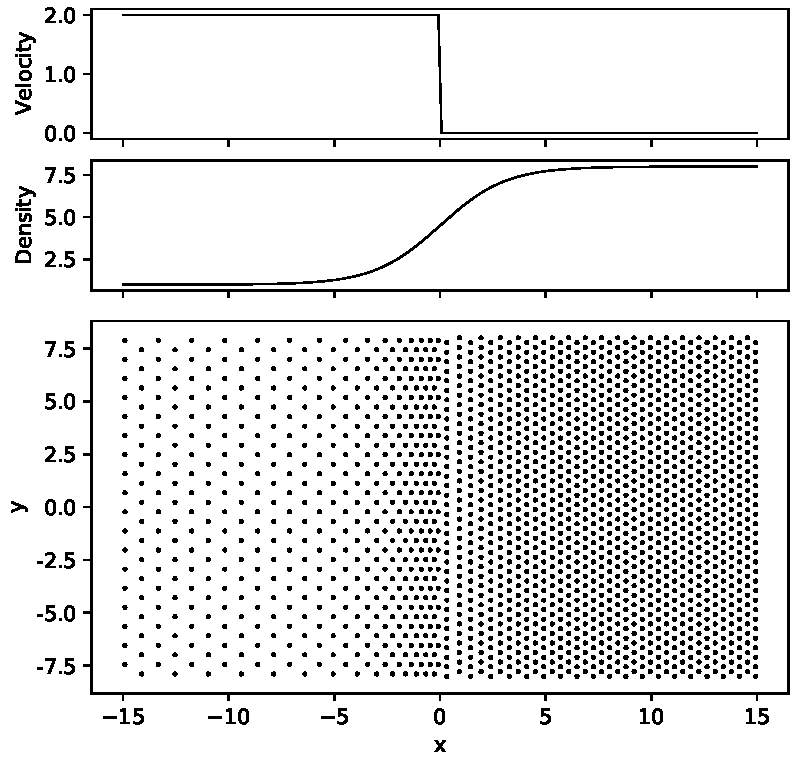
\includegraphics[width=\columnwidth]{figs/dustyshock_initial.pdf}
      \caption{Dusty shock numerical test initial conditions showing the
         velocity (top) and the density (bottom).\label{fig:dustyshock_initial}}
   \end{center}
\end{figure}

\begin{figure*}
   \begin{center}
      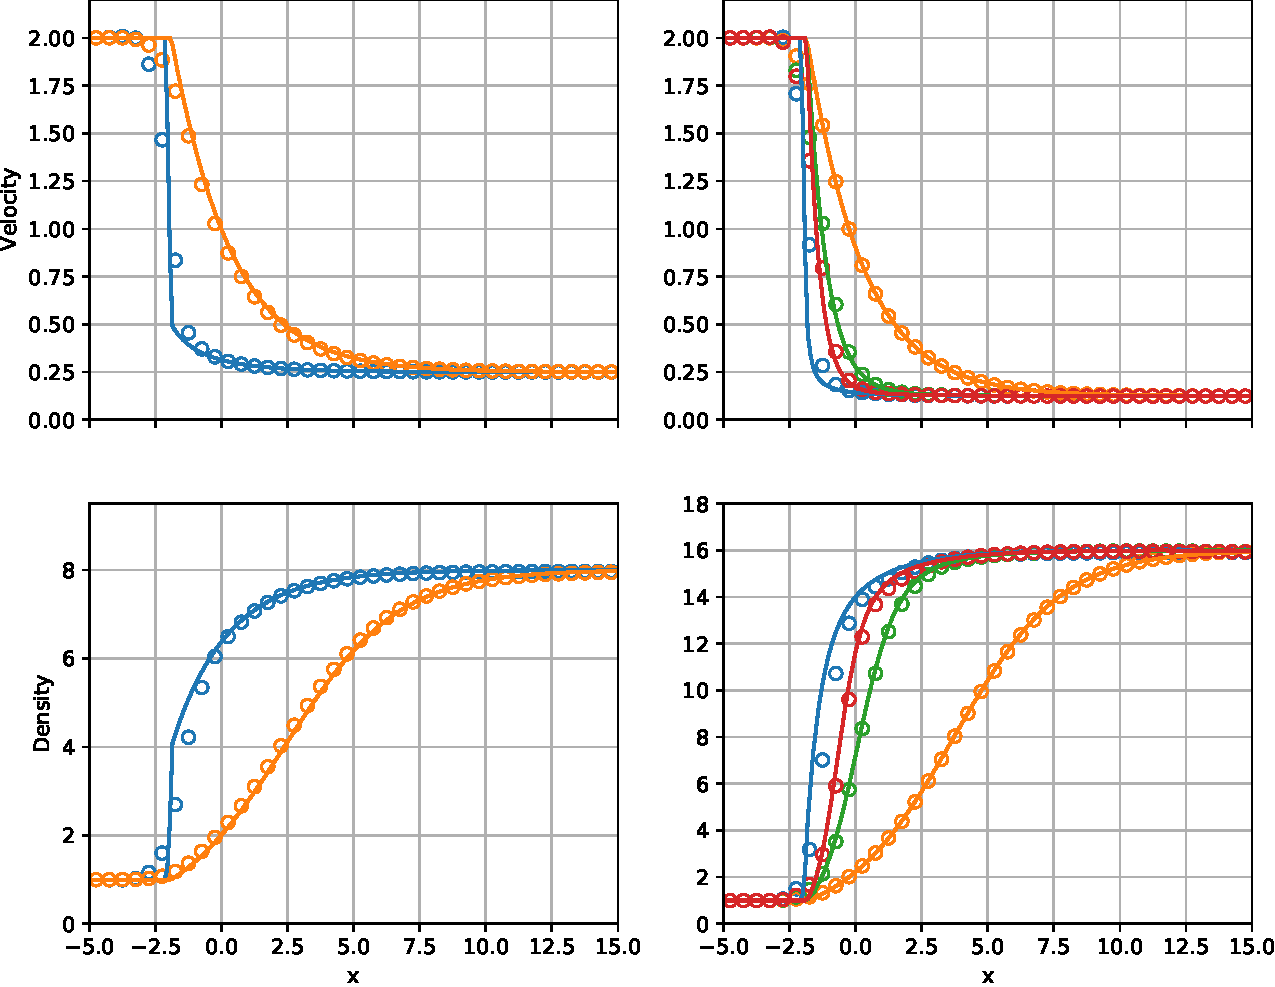
\includegraphics[width=0.66\textwidth]{figs/dustyshock_velocity_density.pdf}
      \caption{Dusty shock numerical test showing the velocity (top) and the
         density (bottom) at time \(t=300\). The left figures have gas (in blue)
         and one dust species; the right figures have gas (blue) and three dust
         species. The open circles represent the results from the
         \textsc{Phantom} simulation. The solid lines represent the analytical
         solution from
         \citet{Benitez-Llambay2019ApJS..241...25B}.\label{fig:dustyshock_final}}
   \end{center}
\end{figure*}

We performed the multiple dust species version of the dusty shock test
described, for the single dust species, in \citet{Laibe2012MNRAS.420.2345L} with
exact solution described in \citet{Lehmann2018MNRAS.476.3185L}. We compare our
numerical solution with the multiple species exact solution
\citep{Benitez-Llambay2019ApJS..241...25B}. The solution is for a steady state
shock described by the following set of equations:
%
\begin{align}
   \frac{\partial}{\partial x} \left( \rho_g v_g \right) &= 0, \\
   \frac{\partial}{\partial x} \left( \rho_{\dd_i} v_{\dd_i} \right) &= 0, \\
   \frac{\partial}{\partial x} \left[ \rho_g (v_g^2 + c_s^2)\right] &= - \sum_{i=1}^N K_i (v_g - v_{\dd_i}), \\
   \frac{\partial}{\partial x} \left( \rho_{\dd_i} v_{\dd_i}^2 \right) &= K_i (v_g - v_{\dd_i}).
\end{align}
%
We use a constant drag coefficient, \(K_i\) per species.

We set up two tests. One test with a single dust species to validate against
previous work. And one test with three dust species to validate our multiple
dust species method. We use that same parameters as
\citet{Benitez-Llambay2019ApJS..241...25B}; see their Table~3.

We set up initial conditions as shown in Figure~\ref{fig:dustyshock_initial}.
\textcolor{red}{(Should this figure be of the particles?)} For the gas and each
dust species, we set up the particles on two close-packed lattices, one on each
side of a discontinuity in the density and velocity in the x-direction with
values on either side of the shock set by their asymptotic values. We use the
same resolution for the gas and each dust species. Due to the
resolution-follows-the-mass nature of SPH, the numerical resolution is higher in
the high density region. \textcolor{red}{Add number of particles.} We smoothed
the density distribution, but not the velocity, using a logistic function,
\(f(x) \propto {\left(1 + e^{-k(x-x_{\rm shock})} \right)}^{-1}\). The large (in
principe, infinite) gradient in density at the shock boundary leads to errors in
evolving the dust.

Figure~\ref{fig:dustyshock_final} shows the velocity and density of both tests
at \(t = 300\) which is long enough so that any transient behaviour has died
out. We have binned the particles into 40 bins in the x-direction and calculated
a mass-weighted average for both density and velocity. We have over-plotted the
analytical solution for comparison. Note that the shock position has drifted
from its initial position and we have shifted the analytical solution shock
position to minimise the error. Our numerical method reproduces the exact
solution in this non-linear test problem.

To achieve an accurate solution we used a larger number of particle neighbours
in the SPH density sum than is typical in dust-gas simulations with
\textsc{Phantom}. The typical neighbour number for quintic kernel, used by
default for dust, density sums in \textsc{Phantom} is 113
\citep{Price2018PASA...35...31P}. The mean neighbour number \(\overline{N}_{\rm
neigh}\) is related to the proportionality constant \(h_{\rm fact}\) by
%
\begin{align}
   \overline{N}_{\rm neigh} = \frac{4}{3} \pi
   {\left( R_{\rm kern} h_{\rm fact} \right)}^3.
\end{align}
%
For the quintic kernel, \( R_{\rm kern} = 3.0 \). So, by default, \( h_{\rm
fact} = 1.0 \).

Figure~\ref{fig:dustyshock_hfact} shows the comparison between the analytical
and numerical solutions for the density varying the value of \( h_{\rm fact} =
1.2, 1.5, 1.8 \), corresponding to \(\overline{N}_{\rm neigh} = 195, 381, 660\).
We can see that the accuracy of the gas density is independent (or only weakly
dependent) on the neighbour number. In contrast, the dust density depends
strongly on the neighbour number. We require \( h_{\rm fact} = 1.5\), for the
single dust species case, and \(h_{\rm fact} = 1.8\), for the three dust species
case.


\section{Discussion}%
\label{sec:discussion}

\begin{figure*}
   \begin{center}
      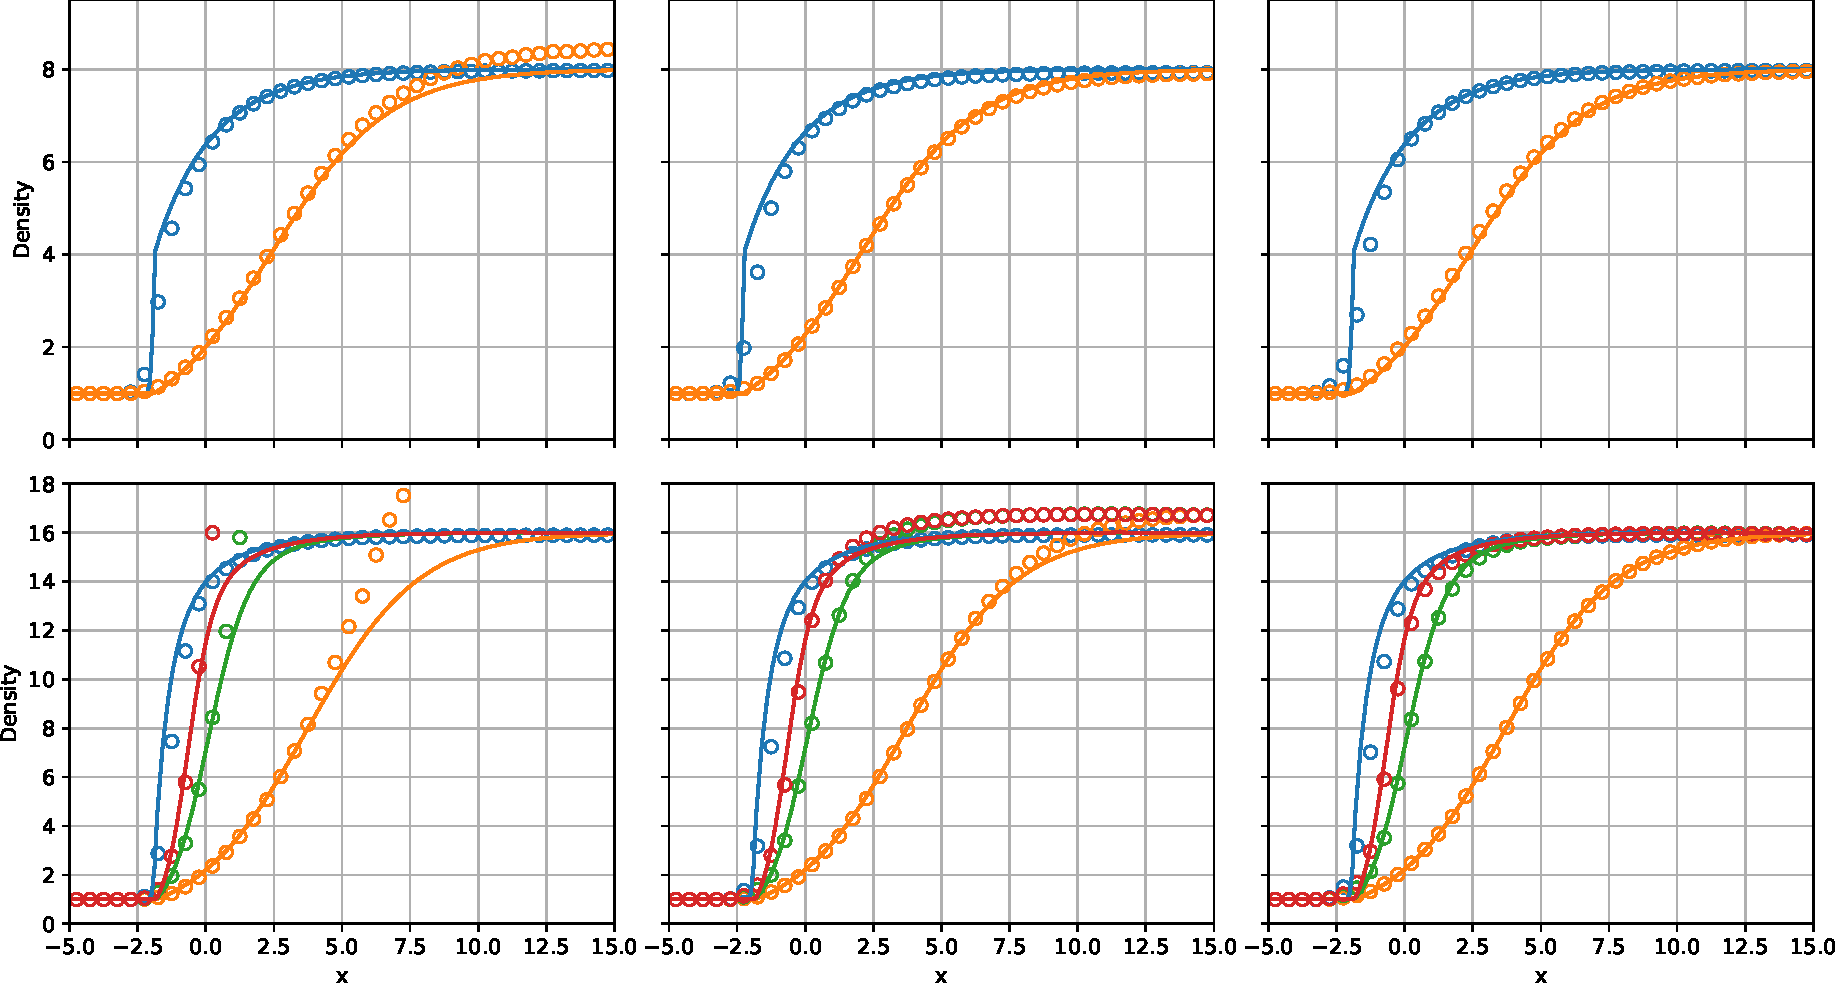
\includegraphics[width=\textwidth]{figs/dustyshock_hfact.pdf}
      \caption{The effect of \(h_{\rm fact}\) in the dusty shock test problem.
         The lines and markers are the same as for \ref{fig:dustyshock_final}.
         From left to right: \(h_{\rm fact} = 1.2, 1.5, 1.8\), corresponding to
         \(\overline{N}_{\rm neigh} = 195, 381,
         660\).\label{fig:dustyshock_hfact}}
   \end{center}
\end{figure*}


\section{Conclusions}


\section*{Acknowledgements}

We used \textsc{Phantom} to perform the numerical simulations
\citep{Price2018PASA...35...31P}. We used \textsc{Plonk} for analysis and
visualisation of \textsc{Phantom} data \citep{Mentiplay2019JOSS....4.1884M}. DM
is funded by a Research Training Program Stipend from the Australian government.
We acknowledge Australia Research Council funding via DP180104235, FT130100034,
and FT170100040. We used OzStar, funded by Swinburne University of Technology
and the Australian government, for computation.


%%%%%%%%%%%%%%%%%%%%%%%%%%%%%%%%%%%%%%%%%%%%%%%%%%

%%%%%%%%%%%%%%%%%%%% REFERENCES %%%%%%%%%%%%%%%%%%

% The best way to enter references is to use BibTeX:

\bibliographystyle{mnras}
\bibliography{multigrain-paper}


%%%%%%%%%%%%%%%%%%%%%%%%%%%%%%%%%%%%%%%%%%%%%%%%%%

%%%%%%%%%%%%%%%%% APPENDICES %%%%%%%%%%%%%%%%%%%%%

% \appendix

% \section{Some extra material}


%%%%%%%%%%%%%%%%%%%%%%%%%%%%%%%%%%%%%%%%%%%%%%%%%%


% Don't change these lines
\bsp % typesetting comment
\label{lastpage}
\end{document}
% End of mnras_template.tex
